\section{Decadimenti nucleari}
La formula semi-emipirica di massa, equazione \ref{formula_semiempirica_massa} nei capitoli precedenti, esprime la stabilità o instabilità dei nuclei nel caso in cui ci sia un'abbondanza di neutroni o di protoni.
Per basi numeri atomici il numero di protoni e di neutroni si equivale, aumentando il numero di massa i nuclei tendono ad avere più neutroni che protoni ed in particolare i nuclei stabili e arrivano ad un numero atomico di circa 80 ed un numero di neutroni di circa 110.
Tutti gli atomi con elevato numero atomico e di massa sono instabili, come ad esempio l'uranio che ha numero atomico 92 ed è un elemento instabile che si trova in natura.
\begin{figure}[h]
\centering
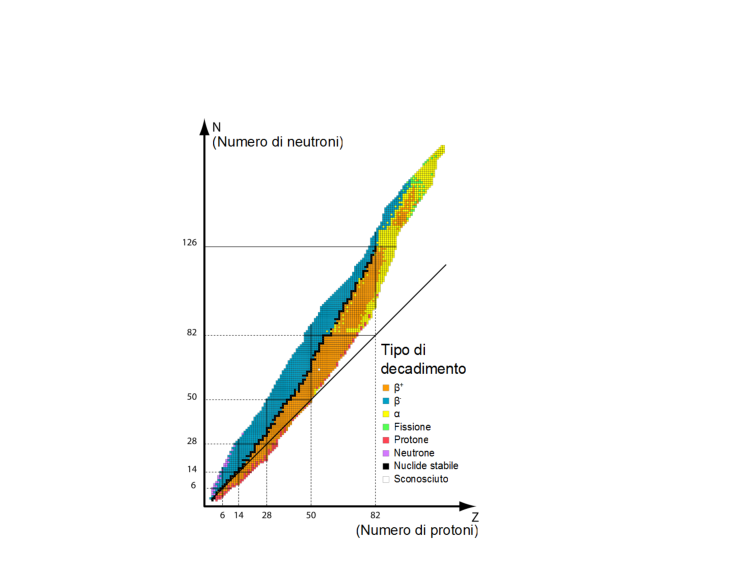
\includegraphics[scale=1]{/nuclei_stabili}
\caption{Il grafico rappresenta per quali combinazioni di neutroni e protoni si hanno atomi stabili.}
\end{figure}
Il decadimento dei nuclei avviene spontaneamente in alcune circostanze

\begin{enumerate}
\item  il nucleo ha troppi neutroni, allora si ha un processo di decadimento beta $\beta^-$
\begin{equation}
^{A}_{Z}X \quad\longrightarrow\quad  ^{A}_{Z+1}X + e^- + \bar\nu_e
\end{equation}
dopo il decadimento si ha un atomo della stessa specie X.
Questo processo è descritto in dettaglio da un decadimento di un neutrone
\begin{equation}
n \quad\longrightarrow\quad p + e^- + \bar\nu_e
\end{equation}
a livello di quark tale processo consiste nella conversione di un quark down in un quark up
\begin{equation}
d \quad\longrightarrow\quad u + e^- + \bar\nu_e
\end{equation}
mediato dal bosone $W$, mediatore della forza debole.

\item il nucleo può avere troppi protoni, si ha allora un processo di decadimento beta $\beta^+$
\begin{equation}
^{A}_{Z}X \quad\longrightarrow\quad ^{A}_{Z-1}Y + e^+ + \nu_e
\end{equation}
dopo il decadimento si ha un atomo di una diversa specie atomica.
Nel dettaglio vediamo che questo processo è descritto dal decadimento di un protone
\begin{equation}
p \quad\longrightarrow\quad n + e^+ + \nu_e
\end{equation}
e a livello di quark 
\begin{equation}
u \quad\longrightarrow\quad d + e^+ + \nu_e
\end{equation}

\item se ci sono troppi nucleoni, quindi siamo nella parte alta del grafico, i nuclei tendono a subire un processo di decadimento alpha $\alpha$, una particella alpha è un nucleo di Elio
\begin{equation}
^{A}_{Z}X \quad\longrightarrow\quad ^{A-4}_{Z-2}Y + \alpha
\end{equation}

\item il nucleo potrebbe avere anche troppa energia, quindi nel caso di un nucleo eccitato $X^{\ast}$, si ha emissione di radiazione elettromagnetica chiamata \emph{radiazione gamma}
\begin{equation}
^{A}_{Z}X^{\ast} \quad\longrightarrow\quad ^{A}_{Z}X + \gamma
\end{equation}

\item nel caso in cui le energie di eccitazione siano molto elevate si può avere decadimento per \emph{fissione} 
\end{enumerate}

Le leggi che descrivono un decadimento impongono la conservazione di 
\begin{itemize}
\item energia
\item quantità di moto
\item carica elettrica
\item numero di nucleoni
\item numero di leptoni
\end{itemize}
la massa invece non si conserva nei processi di decadimento.

\paragraph{esempio} utilizzando la formula semi-empirica di massa si verifichi se il decadimento $\alpha$ del $^{238}_{92} U$ sia possibile energeticamente.

La massa totale iniziale del sistema deve essere maggiore della massa totale finale, allora il processo è esotermico.
$$ M_i > M_f \quad\Rightarrow\quad esotermico $$
\begin{equation}
^{238}_{92} U \quad\longrightarrow\quad ^{234}_{90}X + ^{4}_{2}He
\end{equation}
(l'elemento figlio di questa reazione è un isotopo del Torio $^{232}_{90}Th$, ma non è importante ai fini della trattazione)
dobbiamo calcolare il $Q$ della reazione e ci chiediamo se è maggiore di zero
\begin{equation}
Q = M(A,Z) - M(A-4,Z-2) - M(^{4}_{2}He^{++}) > 0
\end{equation}
la massa dell'atomo iniziale equivale a
\begin{equation}
M(A,Z) = Z M_H + (A-Z)M_n - B(A,Z)
\end{equation}
dove $B$ rappresenta l'energia di legame
quindi il calore nella reazione è
\begin{equation}
\begin{split}
Q  & = -B(A,Z) + B(A-4,Z-2) + B(^{4}_{2}He^{ ++ }) \\
& = [ -1807.5 + (1784 + 32.85)] MeV = \SI{9.35}{MeV} > 0
\end{split}
\end{equation}
risulta quindi positivo, per cui il decadimento alpha è energeticamente possibile, anzi avviene spontaneamente; questo calcolo non ci dice nulla però sulla probabilità che avvenga.
La natura tende a minimizzare la massa.

Ci si può divertire con un programma in MathLab delle slide calcolando l'energia di legame per tutti i nuclei...
si trova l'andamento del calore Q emesso/assorbito dalla reazione in funzione del numero atomico, vedi figura \ref{calore_vs_numatomico}
\begin{figure}[h]
\centering
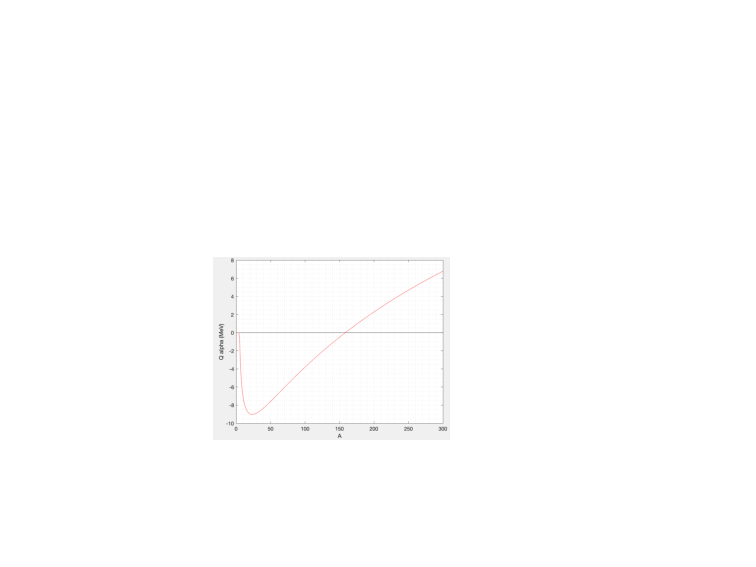
\includegraphics[scale=3]{/calore_vs_numatomico}
\caption{Andamento del calore in funzione del numero atomico}
\label{calore_vs_numatomico}
\end{figure}

\paragraph{esempio} si verifichi se l'Uranio $^{238}_{92}U$ possa decadere $\beta^-$
\begin{equation}
^{238}_{92}U \quad\longrightarrow\quad ^{238}_{92}U 
\end{equation}
ovvero ci si chiede se il calore della reazione è maggiore di zero
\begin{equation}
\begin{split}
Q & = M(A,Z) - M(A,Z+1) > 0 \\
& = -B(A,Z) + B(A,Z+1) + (M_H - M_n) \\
& = -1807.5 + 1805 + (-0.78) = - \SI{3.28}{MeV} < 0
\end{split}
\end{equation}
l'uranio non decade spontaneamente $\beta^-$.


\subsection{Legge del decadimento radioattivo}
Il numero di decadimenti al secondo è proporzionale al numero di atomi contenuti nel campione.
$$\frac{decad}{s} \propto atom$$
Introduco la \emph{costante di decadimento} $\lambda$, che mi permette di riscrivere la formula precedente come
\begin{equation}
\frac{dN}{dt} = - \lambda N
\end{equation}
questa è un'equazione differenziale risolvibile tramite separazione delle variabili
\begin{equation}
\begin{split}
\frac{dN}{N} & = - \lambda dt \\
\ln N & = -\lambda t + C \\
N & = e^{-\lambda t + C} = e^{-\lambda t } e^C 
\end{split}
\end{equation}
trovo la costante di integrazione $C$, imponendo che al tempo $t=0$ il numero totale di atomi sia $N=N_0$,
quindi ottengo $N_0 = 1 e^C$, da cui scriverò
\begin{equation}
N = N_0 e^{-\lambda t} 
\label{eq_decad}
\end{equation}

Il decadimento viene descritto anche da altre quantità, come il \emph{tempo di dimezzamento} $T_{1/2}$: cioè il tempo dopo il quale il numero di neuclidi iniziali si è dimezzato, ovvero $N = N_0 / 2$ e quindi $t= T_{1/2}$
\begin{equation}
\begin{split}
& \frac{N_0}{2} = N_0 e^{-\lambda T_{1/2}} \\
& 2 = e^{ \lambda T_{1/2} } \\
& T_{1/2} = \frac{\ln 2}{\lambda} \simeq \frac{0.693}{\lambda}
\end{split}
\end{equation}
questo tipo di decadimento esponenziale è un processo puramente quantistico, un essere vivente non ha questi problemi... (lol)

Un'altra quantità importante è detta \emph{vita media} $\tau$: 
\begin{equation}
\begin{split}
\tau & = \frac{\int_{N_0}^{0} t dN}{N_0}  = \frac{1}{N_0} \int_0^{\infty} t (-\lambda N_0 e^{ -\lambda t })dt \\
& = - \lambda \Bigl[  \frac{t (-e^{-\lambda t})}{\lambda} - \int \frac{(1) (-e^{ -\lambda t })}{\lambda} \Bigr]_0^{\infty} \\
& = - \lambda \Bigl[  \frac{- t e^{-\lambda t}}{\lambda} - \frac{ e^{ -\lambda t }}{\lambda^2} \Bigr]_0^{\infty} \\
& = \frac{1}{\lambda}
\end{split}
\end{equation}
per cui la vita media corrisponde all'inverso della costante di decadimento e anche a
\begin{equation}
\tau = \frac{1}{\lambda} = \frac{T_{1/2}}{\ln 2} = 1.44 \cdot T_{1/2}
\end{equation}
che corrisponde al momento in cui il numero di neuclidi è sceso al $37\%$ rispetto al valore iniziale.

È da notare che essendo questo un fenomeno quantistico è quindi anche casuale, ciò che sappiamo è che \emph{mediamente} decadono una certa quantità di nuclei ma non sappiamo quali ne quando succederà.
Il tempo di decadimento è indipendente dalla vita del nucleo, per cui esso può decadere immediatamente oppure non decadere mai. 
Ciò differisce nettamente dallo studio di sistemi biologici, che seguono regole più deterministiche.
Seguendo la \ref{eq_decad}, se ci si aspetta $\Delta N $ eventi in un secondo, tale numero di eventi potrà variare, statisticamente rispetto alla media, seguendo la statistica di Poisson in un intervallo dato da
\begin{equation}
\Delta N - \sqrt{\Delta N} < \Delta N < \Delta N + \sqrt{\Delta N}
\end{equation}
nel $67\%$ dei casi il numero di decadimenti sarà compreso in questo intervallo, ma non è una grandezza deterministica.

\paragraph{esempio} supponiamo di avere $10^{12}$ nuclei con una vita media di $\tau = \SI{e10}{s}$, 
quanti decadimenti si hanno in un secondo?
\begin{equation}
\frac{10^{12}}{10^{10}} - \sqrt{\frac{10^{12}}{10^{10}} } < \Delta N < \frac{10^{12}}{10^{10}} + \sqrt{\frac{10^{12}}{10^{10}} } \quad\Rightarrow\quad 90 < \Delta N < 110
\end{equation}
abbiamo in questo caso una precisione del $10\%$.

Nei processi di decadimento molto rari si utilizza la statistica di Poisson.
\paragraph{esempio} se ho $\Delta n$ al secondo che probabilità ho di registrare $K$ eventi? (se $\Delta n$ è piccolo, con bassa costante di decadimento)
La probabilità in questo caso è data dalla statistica di Poisson
\begin{equation}
P(\Delta n, K) = \frac{\Delta n^K}{K!} e^{ -\Delta n }
\end{equation}

\subsection{Catene di decadimento}
Normalmente i decadimenti avvengono in cascata e sono dominate da un sistema di equazioni differenziali, tali equazioni sono chiamate \emph{equazioni di Bateman}
\begin{equation}
\begin{split}
& \frac{dN_1}{dt} = - \lambda_1 N_1(t) \\
& \frac{dN_2}{dt} = - \lambda_1 N_1(t) - \lambda_2 N_2(t) \\
& \frac{dN_i}{dt} = - \lambda_{i-1} N_{i-1}(t) - \lambda_i N_i(t) \\
& \frac{dN_k}{dt} = - \lambda_{k-1} N_{k-1}(t)
\end{split}
\label{bateman_equations}
\end{equation}

\paragraph{esempio} Un nucleo di Uranio che fa \emph{fissione} si divide in due nuclei che hanno circa la metà del numero di massa iniziale. I prodotti di fissione sono radioattivi perché il numero di neutroni è maggiore di quello della stabilità in quanto arrivano da un nucleo con un grande numero di massa.











